\subsection*{Material Correspondence Table}
I reconstructed the original study material by dividing some parts into smaller sections to make a step-by-step approach to the content in the notes. \smallskip

\noindent And, since this chapter is about "preliminaries", I would not dig too deep into the stated concepts, properties and detailed proofs. The material here is more designed to help you recap the basics of linear algebra, and you might see a lack of correspondence between sections and exercises.
\smallskip

\noindent If you want to see the correspondence of the materials between the original and commentary notes, here is a table indicating the relations: \bigskip

\noindent 
\begin{tabular}{ll}
  Master Notes & Commentary Notes \\
  \hline \\
  1.1. Matrices, vectors and matrix-vector multiplication & Section 1.1 - 1.3 \\
  1.2. Range, nullspace and rank & Section 1.4 - 1.6 \\
  1.3. Invertibility and inverses & Section 1.7  \\
  1.4. Adjoints and Hermitian matrices & Section 1.8 \\
  1.5. Inner products and orthogonality & Section 1.9 \\
  1.6. Orthogonal components of a vector & Section 1.10\\
  1.7. Unitary matrices & Section 1.11  \\
  1.8. Vector norms & Section 1.9\\
  1.9. Projectors and projections &  Section 1.12 \\
  1.10. Constructing orthogonal projectors  & Section 1.13
  \end{tabular}
\newpage
\section{Matrix-Vector Multiplication}%
\textbf{This part might be too easy for most of you - but it would still give you intuition in the contents we would discuss later.}\medskip

\noindent Note that in this course we would discuss \textbf{vectors in \(\mathbb{C}^{n}\) rather than \(\mathbb{R}^{n}\)}, so some vector operations would be different from those you get used to. You would see the details as we go through the course.
% \subsection*{Content Checklist}
% \noindent In this section we would:
% \begin{itemize}
%   \item Recap on \textbf{Matrix-Vector multiplication formula}. 
%   \item \textbf{Implement a Python function} for M-V multiplication.
% \end{itemize}
\subsection*{Contents}
\begin{definition}[Matrix-Vector Multiplication]
  Suppose we are given that:
  \[
    x = \begin{pmatrix} x_1\\x_2\\ \vdots\\ x_n \end{pmatrix} \in \mathbb{C}^{n} \text{ and } 
      A = \begin{pmatrix} 
      a_{11} & a_{12} & \ldots & a_{1n} \\
    a_{21} & a_{22} & \ldots & a_{2n} \\ 
    \vdots & \vdots & \ddots & \vdots \\
    a_{m1} & a_{m2} & \ldots & a_{mn} \\  
    \end{pmatrix} \in \mathbb{C}^{m \times n}
  .\] 
  The problem asked to compute the value of $b = Ax$ is called the \textbf{Matrix-Vector} multiplication problem, where
  \[
    b_i = \sum_{j = 1}^{n} a_{ij}x_j, \text{ where } i \in \{1, 2, 3 \ldots m\} 
    .\checked\] 
\end{definition}
This operation, or we say the map $x \to  Ax$ is indeed a linear map from $\mathbb{C}^{n} \to \mathbb{C}^{m}$. 
This should be really straightforward for you and I would skip the proof. \medskip

\noindent Now you can compute the \(i\)the entry \(b_i\) from the formula above. Consider how you normally compute the value of \(b\), and how to use this schema further to implement a python function. Try exercise 1.1 to see if you could convert the math to executable code.
\subsection*{Exercise 1.1: Basic M-V Multiplication}
\addcontentsline{toc}{subsection}{Exercise 1.1: Basic M-V Multiplication}
\begin{problem}
  Given matrix $A$ and vector $x$ as defined above, you need to implement a function \href{https://comp-lin-alg.github.io/cla_utils.html#cla_utils.exercises1.basic_matvec}{\texttt{exercises1.basic\_matvec()}}
under the \texttt{cla\_utils} package, which returns the matrix-vector product $b = Ax$.
\end{problem}
\noindent I would give you some instructions in this exercise:
\begin{enumerate}
  \item Clearly to compute the value of \(b\)  we need to compute all \(m\)  entries \textbf{repeatedly}, just like what we normally do with paper and pens. So a \textbf{for} loop in the form \texttt{for i in range(m)} is required. In this loop, we compute \(b_i\) for each value of \(i\).
  \item To compute \(b_i\), we apply the formula with summation variable \(j\). You should see we need another \textbf{for} loop in the form \texttt{for j in range(n)} to compute \(b_i\)  , since \(j\) is changing from 1 to n in the formula. 
  \item When computing \(b_i\), what you need to do is just keep adding summation components, and finally store the value into your final \(b\). \checked
\end{enumerate}
The instructions should be clear enough for you to start the very first exercise. The most naive structure of code should be:
\begin{lstlisting}[language=Python]
import numpy as np
def basic_matvec(A, x):
    # Get the dimensions of A
    m, n = ...
    # Initialise vector b as a zero vector.
    b = np.zeros(n)
    for i in range(m):
        b_i = 0
        # Compute the value of b_i.
        for j in range(n):
            # Apply the basic formula in summation.
            b_i += ...
        # set the ith entry of b as b_i.
        b[i] = b_i
    return b
\end{lstlisting}
\textbf{Make sure your code implementation passes the provided test cases.}
\section{Column-Space Formulation}
\label{sec1.2}
In this section, we would give you an intuition to interpret matrix-vector multiplication as a linear combination of columns of $A$, with coefficients taken from the entries of $x$.
% \subsection*{Content Checklist}
% \noindent In this section we would:
% \begin{itemize}
%   \item Introduce the concept of \textbf{Column-Space Formulation}. 
%   \item \textbf{Implement a Python function} for M-V multiplication with C-S Interpretation.
% \end{itemize}
\subsection*{Contents}
\begin{definition}[Column-Space Formulation]
  Suppose we have matrix \(A\)  in the form
  \[
    A = \begin{pmatrix}
      a_1 & a_2 & \ldots & a_n
    \end{pmatrix}
  .\]
  The result of \(b = Ax\)  is a linear combination of columns of \(A\), \(a_i\)  with the entries of \(x\)  as coefficients. i.e.
  \[
    b = Ax =  \sum_{i=1}^{n} x_i a_i
  .\]
\end{definition}
\begin{explanation}
  We firstly ignore the special form of \(A\) with column notation, and use the basic M-V multiplication formula to expand \(b\):
  \[
b = \begin{pmatrix} a_{11}x_1 + a_{12}x_2 + \cdots + a_{1n}x_n \\  a_{21}x_1 + a_{22}x_2 + \cdots + a_{2n}x_n\\ \vdots\\a_{m1}x_1 + a_{m2}x_2 + \cdots + a_{mn}x_n \end{pmatrix}
\]
Indeed this is equivalent to
\[
b = x_1\begin{pmatrix} a_{11}\\ a_{21} \\ \vdots\\ a_{m1} \end{pmatrix} + x_2 
\begin{pmatrix} a_{12}\\ a_{22} \\ \vdots\\ a_{m2} \end{pmatrix} + \cdots + x_n 
\begin{pmatrix} a_{1n}\\ a_{2n} \\ \vdots\\ a_{mn} \end{pmatrix}
.\]
Then we apply the special column notation \(a_i = \begin{pmatrix} a_{1i} & a_{2i} & \ldots & a_{mi} \end{pmatrix}^{\top}\) and we should get
\[
  b = x_1a_1 + x_2a_2 + \cdots + x_na_n = \sum_{j=1}^{n} x_j a_j
.\]
with \(b\) as a linear combination of columns of \(A\) and entries of $x$. 
\end{explanation}

\begin{note}
  You could see now that \(b\)  is spanned by columns of \(A\), and that is why we called it Column-Space Formulation (or Interpretation).
\end{note}

\subsection*{Exercise 1.2: M-V Multiplication with C-S Formulation}%
\addcontentsline{toc}{subsection}{Exercise 1.2: M-V Multiplication with C-S Formulation}
\begin{problem}
  We were still considering to compute the value of \(b = Ax\), but now you are asked to implement a function \href{https://comp-lin-alg.github.io/cla_utils.html#cla_utils.exercises1.column_matvec}{\texttt{column\_matvec()}} with \textbf{exactly one loop} over entries of \(A\) (and \(x\)).
\end{problem}
\noindent You might find the column-space formulation we mentioned above is helpful for implementation, i.e.:
\[
b = Ax =  \sum_{i=1}^{n} x_i a_i
.\]

\begin{hint} 
Here are several things also worth mentioning:

\begin{enumerate}
\item Since we are asked to use a \textbf{single loop} only, we could easily see that using the formula above with one $\Sigma$ sign would work. 
\item Then what you need to do is just add up the multiples of column vectors in the loop. Make sure you know how to get the \(i\)th column vector from \(A\)  in \texttt{numpy}. \checked
\end{enumerate}
\textbf{Make sure your implementation passes the provided test cases.}
\end{hint}

\section{Matrix-Matrix Multiplication}%
\label{sec1.3}
% \subsection*{Content Checklist}
% \noindent In this section we would:
% \begin{itemize}
%   \item Extend the multiplication formula for the \textbf{Matrix-Matrix} Case.
%   \item Recap and extend the \textbf{outer} and \textbf{inner} product of vectors in \(\mathbb{C}^{m}\).
%   \item Compare the \textbf{execution time} of M-V multiplication with \textbf{different implementations}.
% \end{itemize}
\subsection*{Contents}
\begin{definition}[Matrix-Matrix Multiplication]
  Suppose we are given $A \in \mathbb{C}^{m \times l}m C \in \mathbb{C}^{l \times n}$, to compute matrix $B = AC$ we have:
  \[
    b_{ij} = \sum_{k = 1}^{l} a_{ik}c_{kj} 
  .\]  
\end{definition}
\begin{note}
  If we consider the relation between the \(i\)th column of \(B\) and \(C\), \(b_i\)  and \(c_i\), you would see
  \[
    b_i = Ac_i
  .\]
  which means the \textbf{\(i\)th column} of \(B\) is the \textbf{matrix-vector product} of A with the \textbf{\(i\)th column} of \(C\). This is very important for you when understanding the matrix factorisation algorithms in the following chapters. \checked
\end{note}
However, you might consider what would happen if two vector-like matrices multiply together, i.e. multiplication between \(m \times 1\) and \(1 \times m\) matrices. Here we define the \textbf{outer product} for vectors to describe this operation:
\begin{definition}[Outer Products for Real Vectors]
  Suppose \(u, v \in \mathbb{R}^{m}\), the outer product between \(u\) and \(v\) is:
  \[
    uv^{\top} = \begin{pmatrix} 
      uv_1 & uv_2 & \dots & uv_m 
    \end{pmatrix} \in \mathbb{R}^{m\times m}
  .\]
\end{definition}
and we could extend this definition to \textbf{complex vectors}:
\begin{definition}[Outer Products for Complex Vectors]
  Suppose \(u, v \in \mathbb{C}^{m}\), the outer product between \(u\)  and \(v\)  is:
  \[
    uv^{*} = \begin{pmatrix} 
      u\overline{v_1} & u\overline{v_2} & \dots & u\overline{v_m}
    \end{pmatrix} \in \mathbb{C}^{m \times  m} 
  .\]
  where \(v^{*}\) is the complex conjugate of \(v^{\top}\).
\end{definition}     
The \(^{*}\) sign is also widely used in finding adjoints of complex matrices. We would discuss the properties further in \autoref{sec1.7}. \smallskip

\noindent And we have also defined \textbf{inner product} which gives out a scalar:
\begin{definition}[Inner Products for Complex Vectors]
  Suppose \(u, v \in \mathbb{C}^{m}\), the inner product between \(u\)  and \(v\)  is:
  \[
    u^{*}v = \sum_{i=1}^{m} \overline{u_i}v_i \in \mathbb{C}
  .\] 
\end{definition}   
\begin{property}
  The inner product is bilinear. Try to prove this property.
\end{property}
The concept of the inner product is strongly related to the orthogonality and norm of vectors. We would discuss the concepts further in \autoref{sec1.8}. \checked
\subsection*{Exercise 1.3: Execution Time Comparison}%
\addcontentsline{toc}{subsection}{Exercise 1.3: Execution Time Comparison}
You don't need to implement anything in this exercise, but just run several lines of code in your terminal. \textbf{This exercise is not assessed.}
\begin{problem}
Now you have two equivalent implementations of matrix-vector multiplication, and we want to see how fast these two and the default \texttt{numpy} implementation could handle the matrix-vector problem. 

\noindent Use the pre-defined function $\texttt{time\_matvecs()}$ to see the execution time among the following implementations:
\begin{lstlisting}
> basic_matvec(A0, x0) # double-nested loop implementation

> column_matvec(A0, x0) # single loop implementation

> A0 @ x0 # using @ ("at" sign) as matmul operator in numpy
\end{lstlisting}
\end{problem}
\subsubsection*{Efficiency Measuring}
Run the following code in your terminal and you could see that:
\begin{lstlisting}
>>> import cla_utils
>>> cla_utils.time_matvecs()
Timing for basic_matvec
0.09208189499999975
Timing for column_matvec
0.002095079000000055
Timing for numpy matvec
0.00014622799999841618
\end{lstlisting}
All methods should be equivalent, but as for the execution time:
\[
\texttt{basic} \gg \texttt{column-space} \gg \texttt{numpy implementation}
.\]
This is because \texttt{numpy} optimised the efficiency in general numerical operations. Therefore, in this course you are always recommended to use basic \texttt{numpy} functions other than your own implementation, except in the case you are not allowed to use some functions e.g. \texttt{np.linalg.qr()}. \checked
\section{Range of a Matrix}%
\label{sec1.4}
% \subsection*{Content Checklist}
% \noindent In this section we would:
% \begin{itemize}
%   \item Introduce the concept of \textbf{range}.
%   \item Relate range of matrix to the \textbf{span} of column vectors. 
% \end{itemize}
\subsection*{Contents}
\begin{definition}[Range of a Matrix]
  Suppose \(A \in \mathbb{C}^{m \times n}\), the range of \(A\) is defined as:
  \[
  \text{range}(A) = \{a : \exists x \in \mathbb{C}^{n}, Ax = a \}
  .\checked\]
\end{definition}
One interesting conclusion about the range is:
\begin{prop}[range is equal to the span of column vectors]
  \[
    \text{range}(A) = \text{span}(a_1, \cdots, a_n)
  .\] 
  i.e. range($A$) is the vector space spanned by the columns of $A$.
\end{prop}
This is obvious to see. Let me explain it a little bit. 

\noindent Since any vector \(a \in\) range\((A)\)  is in the form \(Ax\), i.e. any vector in range of \(A\)  is a linear combination of column vectors of \(A\), and it would also be in the vector space spanned by column vectors.

\noindent Also, since any vector in the span of column vectors is a linear combination of the columns, it should also be an element of range($A$), our job is done. \checked


\section{Null Space and Rank of a Matrix}%
\label{sec1.5}
\subsection*{Content Checklist}
% \noindent In this section we would:
% \begin{itemize}
%   \item Introduce the concept of null space and rank.
%   \item Learn to construct a \textbf{rank-2 matrix} with python.
% \end{itemize}
\subsection*{Contents}
\begin{definition}[Null Space of a Matrix]
  Suppose \(A \in \mathbb{C}^{m \times n}\), the null space of \(A\) is defined as:
  \[
    \text{null}(A) = \{x \in \mathbb{C}^{n}: Ax = 0\} 
  .\]
\end{definition}

\begin{definition}[Rank of a Matrix]
  \[
  \text{rank}(A) = \text{dim}(\text{span}(a_1, a_2, \cdots, a_n)) = \text{dim}(\text{range}(A))
\]
where \(a_i\)  column vectors. 
\end{definition}
\begin{property}
  \(\forall A \in \mathbb{C}^{m \times n}\), rank\((A) \leq \min(m, n)\).
\end{property}
\begin{definition}[Full Rank]
  Suppose \(A \in \mathbb{C}^{m \times n}\), if 
  \[
    \text{rank}(A) = \min(m, n)
  \]
  we say \(A\) has a full rank. \checked
\end{definition}

\subsection*{Exercise 1.11: Construct a Rank-2 Matrix}%
\addcontentsline{toc}{subsection}{Exercise 1.11: Construct a Rank-2 Matrix}
\begin{problem}
  Given that we have $u_1, u_2 \in \mathbb{C}^{m}$ and $v_1, v_2 \in \mathbb{C}^{n}$, we want to construct a rank-2 matrix $A = u_1v_1^{*} + u_2v_2^{*}$. However, from the given code and the specification, we need to implement a function \href{https://comp-lin-alg.github.io/cla_utils.html#cla_utils.exercises1.rank2}{\texttt{exercises1.rank2()}} returning matrix  $A$ as a product of two other matrices $B$ and $C$.
\end{problem}
\begin{hint}
  We need to consider the following two questions:
\end{hint}
\begin{itemize}
  \item How to expand $A$ from outer products?
  \item Can you find the relation between columns of \(A\), \(u\) and \(v\)?
\end{itemize}
Pause here for a moment to think about these two questions. Feel free to read the answers on the next page if you get confused.
\newpage

\noindent Here we consider the $A$ as a summation of two matrices first:
\[
A = u_1v_1^{*} + u_2v_2^{*}
\]
where
\[
  u_1v_1^{*} = \begin{pmatrix} v_{11}^{*}u_1 & v_{12}^{*}u_1 & \cdots & v_{1n}^{*}u_1 \end{pmatrix} 
\]
and
\[
  u_2v_2^{*} = \begin{pmatrix} v_{21}^{*}u_2 & v_{22}^{*}u_2 & \cdots & v_{2n}^{*}u_2 \end{pmatrix} 
.\] 
Therefore, $A$ could be written in the sum:
\[
  A = u_1v_1^{*} + u_2v_2^{*} = \begin{pmatrix} v_{11}^{*}u_1 + v_{21}^{*}u_2 & v_{12}^{*}u_1 + v_{22}^{*}u_2 & \cdots & v_{1n}^{*}u_1 + v_{2n}^{*}u_2 \end{pmatrix} 
\]
with
\[
  a_{i} = v_{1i}^{*}u_1 + v_{2i}^{*}u_2 = \begin{pmatrix} u_1 & u_2 \end{pmatrix} \begin{pmatrix} v_{1i}^{*}\\ v_{2i}^{*} \end{pmatrix}
.\] 
To generalize this, we could now write $A$ in terms of a product of two matrices:
\[
A = \begin{pmatrix} u_1 & u_2 \end{pmatrix} \begin{pmatrix} v_{1}^{*}\\ v_{2}^{*} \end{pmatrix}   = \begin{pmatrix} u_1 & u_2 \end{pmatrix} \begin{pmatrix} v_{1}^{*} & v_{2}^{*} \end{pmatrix}^{\top}
.\]
So our first job has been done, now it is your time for implementation. \medskip

\noindent 
\textbf{Remember to check your implementation pass the provided test cases.}
\subsubsection*{Analysis}
Now let us talk about the rank of $A$, we claim the rank is necessarily 2.
Recall the result of $A$ we have found with the column-space formulation: 
\[
A = u_1v_1^{*} + u_2v_2^{*} = \begin{pmatrix} v_{11}^{*}u_1 + v_{21}^{*}u_2 & v_{12}^{*}u_1 + v_{22}^{*}u_2 & \cdots & v_{1n}^{*}u_1 + v_{2n}^{*}u_2 \end{pmatrix} 
.\]
We could see that every column of $A$ is a linear combination of $u_1$ and $u_2$, assuming that they are linearly independent. Therefore, when we are talking about the range of $A$, it should be a vector space spanned by $u_1$ and $u_2$ and the dimension of the space should be 2. \textbf{i.e. the rank is 2 obviously.} \checked

\section{Invertibility and inverses}%
\label{sec1.6}
The idea and properties related to invertibility and inverses should be quite familiar, I would not talk about the definitions here. 
\section*{Contents}
Consider the matrix-vector equation \(Ax = b\), assume \(A\) is invertible:
\begin{itemize}
  \item From entries of b, we could see the basis coefficients in the canonical basis $\{e_i\}$. 
  \item From the column-space formulation, we could see \(b\) is also a linear combination of columns of \(A\), with entries of \(x\) as basis coefficients and \(\{a_i\}\)  as a basis. 
  \item Therefore, if we find \(x\), we could find a change of basis of \(b\)  from canonical basis to column basis \(\{a_i\}\).
  \item Since \(x = A^{-1}b\), we need to find \(A^{-1}\) to solve \(x\). Therefore we could say finding the inverse of matrix \(A\) can be seen as a change of basis.
\end{itemize}
This might not be relevant to the following exercise, but it would be helpful when you understand orthogonal projectors. \checked
\subsection*{Exercise 1.13: Find the inverse of a given matrix}%
\addcontentsline{toc}{subsection}{Exercise 1.13: Find the inverse of a given matrix}
\begin{problem}
  Given that a square matrix $A = I_m + uv^{*} \in \mathbb{C}^{m \times m}$, where $u, v \in \mathbb{C}^{m}$. Suppose we could find the inverse $A'$ written in  $A' = I_m + \alpha uv^{*}$, determine the value of $\alpha$ and implement the function \href{https://comp-lin-alg.github.io/cla_utils.html#cla_utils.exercises1.rank1pert_inv}{\texttt{rank1pert\_inv()}} to return the inverse matrix $A'$. \medskip
\end{problem}

\noindent Pause here for a moment to think about writing the value of \(\alpha\) in terms of \(u\) and \(v\). Feel free to read the answers on the next page if you get confused.
\newpage
\subsubsection*{What to do}
\noindent So we try to determine the value of $\alpha$ first:
\begin{itemize}
  \item Given that $A A^{-1} = I_m$:
    \[
      A A^{-1} = (I_m + u v^{*})(I_m + \alpha u v^{*}) = I_m + uv^{*} + \alpha uv^{*} + \alpha u v^{*}uv^{*} = I_m
    .\]
  \item Since the inner product, $v^{*}u$ is a scalar, then we could have:
    \[
      uv^{*} + \alpha uv^{*} + \alpha (v^{*}u)uv^{*} = 0_{m \times m} \implies (1 + \alpha + \alpha v^{*}u)uv^{*} = 0_{m \times m}
    .\]
  \item Therefore, we have:
    \[
    \alpha (1 + v^{*}u) = -1 \implies \alpha = -\frac{1}{1 + v^{*}u}
    \]
    and
    \[
    A^{-1} = I_m -\frac{1}{1 + v^{*}u} uv^{*}
    \]
    whenever $A$ is invertible.
\end{itemize}
So the code implementation for you should be very simple. \checked \medskip

\noindent \textbf{Check your implementation passes the provided test cases.}
\subsubsection*{Efficiency Measuring (Non-assessed part for this exercise)}
To measure the time taken for computing the inverse of this implementation, and compare it with the built-in numpy implementation (just like what we did for timing the matrix-vector multiplication), I add the following code:
\lstinputlisting[language=Python, firstline=65, lastline=77]{./python/exercise1.py}
with pre-defined \texttt{u0}, \texttt{v0}, and the output shows that:
\begin{lstlisting}
>>> import cla_utils
>>> cla_utils.time_matinvs()
Timing for basic_matinv
0.0013024520000044504
Timing for numpy matinv
0.005589449000012792
\end{lstlisting}

\noindent We could see that the numpy implementation is slower. The reason for this is, unlike our implementation, the numpy implementation didn't take the advantage of the structure of \(A\) - a rank-2 matrix constructed via \(u\) and \(v\), therefore, the complexity using numpy is greater than our implementation and the time taken is indeed longer.

\section{Adjoints and Hermitian Matrices}%
\label{sec1.7}
% \subsection*{Content Checklist}
% \noindent In this section we would:
% \begin{itemize}
%   \item Introduce the concept of Matrix Adjoints and Hermitian Matrices.
%   \item Coding Exercise with a Hermitian matrix.
% \end{itemize}
\subsection*{Contents}
\begin{definition}[Adjoints of Matrices]
  Suppose \(A \in \mathbb{C}^{m \times n}\), the adjoint (or Hermitian conjugate) \(A^{*} \in \mathbb{C}^{n \times m}\) is defined as:
  \[
    a^{*}_{ij} = \overline{a_{ji}}
  .\]
  which is equivalent to
  \[
    A^{*} = \overline{A^{\top}}
  .\]
\end{definition}
\begin{definition}[Hermitian Matrices]
  \[
    A^{*} = A \Rightarrow A \text{ Hermitian}  
  .\]
\end{definition}
\begin{property}
  \[ 
  (AB)^{*} = B^{*}A^{*}, A \in \mathbb{C}^{m \times n}, B \in \mathbb{C}^{n \times l}
.\] 
\end{property}
Feel free to prove this property.
And then we could look at the following exercise implementing the required function \href{https://comp-lin-alg.github.io/cla_utils.html#cla_utils.exercises1.ABiC}{\texttt{exercises1.ABiC()}}. \checked
\subsection*{Exercise 1.16: Hermitian Matrices and Multiplication}%
\addcontentsline{toc}{subsection}{Exercise 1.16: Hermitian Matrices and Multiplication}
These exercises have several mini-questions for us to solve. The first part is mainly about proof with hermitian matrices, and the function implementation part is about the application. Let's see the proof exercise first.

\subsubsection*{Task 1}%

\noindent Given that $A = B + iC \in \mathbb{C}^{m \times m}$ where $B, C$ are both real matrices with compatible dimensions, and  $A$ is hermitian, show that:
\[
  B = B^{\top} \text{ and } C = -C^{\top}
.\]
\begin{proof}
  Your work (but not assessed).
\end{proof}
\subsubsection*{Task 2}%
We are required to compute the real and imaginary part of the matrix multiplication product $z = Ax$, where  $A$ is defined above. To save memory, the function would not accept the contents of $A$ as an argument, but a modified matrix $\hat{A}$, where
\[
\hat{A}_{ij} = \left\{
  \begin{array}{l}
  B_{ij} \text{ where } i \ge j \\
  C_{ij} \text{ where } i < j.
  \end{array}
\right.
.\] 
Therefore, given a matrix $\hat{A}$ and $x_r, x_i$ where  $x = x_r + ix_i$, we need to implement the function \href{https://comp-lin-alg.github.io/cla_utils.html#cla_utils.exercises1.ABiC}{\texttt{exercises1.ABiC()}} to get the real and imaginary parts of \(z = Ax\). Note that all your matrix-vector multiplication should be done via column-space formulation. \medskip

\noindent Pause here for a moment to think about your implementation step by step. Feel free to read the instructions on the next page if you get confused.
\newpage
\subsubsection*{What to do}
\begin{enumerate}
\item Since we don't have contents of $A = B + iC$ as required, we could first try to get contents in $B$ and $C$ from $\hat{A}$.
\item The contents in $\hat{A}$ should look like this:
  \[
    \hat{A} = \begin{pmatrix} 
      b_{11} & c_{12} & c_{13} & \ldots & c_{1m} \\
      b_{21} & b_{22} & c_{23} & \ldots & c_{2m} \\
      b_{31} & b_{32} & b_{33} & \ldots & c_{3m} \\
      \vdots & \vdots & \vdots & \ddots & \vdots \\ 
      b_{m1} & b_{m2} & b_{m3} & \ldots & b_{mm}
    \end{pmatrix} 
  .\]
  So what we could do is to extract the lower-triangular part of $B$ and upper-triangular part of $C$ from $\hat{A}$, by using \texttt{np.triu()} and \texttt{np.tril()}, and then get the full form of $B$ and  $C$ by transposition.
 \item After having $B$ and $C$, we could simply calculate the value of  $z = Ax$:
    \[
      z = Ax = (B + iC)(x_r + ix_i) = (Bx_r - Cx_i) + i(Bx_i + Cx_r)
   \]
   where $z_r$ and $z_i$ could be easily seen. \checked
\end{enumerate}
\textbf{Remember to check your implementation pass the provided test cases.}
\section{Inner Products, Orthogonality and Vector Norms}%
\label{sec1.8}
The idea of these concepts is very simple but they are extremely important in computational linear algebra. Here I would just focus on definitions to give you an insight.
\subsection*{Contents}
We have seen the definition of inner product in \autoref{sec1.3}, and the definition of 2-norm is based on that:
\begin{definition}[2-norm]
  Suppose \(x \in \mathbb{C}^{m}\), the 2-norm of \(x\) is defined as:
  \[
    \|x\| = \sqrt{\sum_{i=1}^{m} |x_i|^2} = \sqrt{x^{*}x}
  .\]
\end{definition}
And orthogonality is based on inner product and 2-norm:
\begin{definition}[Orthogonality]
  Suppose \(x, y \in \mathbb{C}^{m}\), we say \(x\) and \(y\) are orthogonal if
  \[
    x^{*}y = 0
  .\]
  Similarly, two sets \(X, Y\) are orthogonal if
  \[
    \forall x \in X, y \in Y, x^{*}y = 0
  .\]
  And a set \(S\) is orthogonal itself if
  \[
    \forall x, y \in S,  x^{*}y = 0
  .\]
  A set \(S\) is orthonormal if \(S\) is orthogonal and \(\|x\| = 1 \forall x \in S\).   
\end{definition}
There are also definitions and properties of general norms and weighted norms mentioned in the original notes, but they are not quite relevant to the study material so I won't mention them here. \checked
\bigskip

\begin{center}
  \textit{\large End of Week 1}
\end{center}
\newpage
\section{Orthogonal Components of a Vector}%
Given that we have a orthonormal set of vectors $S = \{q_1, q_2, \ldots, q_n\} $ where $q_i \in \mathbb{C}^{m}$. Now we claim that, for any vector $v \in \mathbb{C}^{m}$, we have:
\begin{prop}[Orthonormal Decomposition]
  \[
  v = r + \sum_{i=1}^{n} (q_i^{*}v)q_i = r + \sum_{i=1}^{n} (q_iq_i^{*})v
.\]
where \(r\) orthogonal to any \(q_i \in S\).
\end{prop}
This is easy to see, you can check by rewriting \(r\)  in terms of \(v\)  and \(q_i\), and compute the value of the inner product between r and an arbitrary \(q_i\). \smallskip

\noindent This proposition is also important since it shows us:
\begin{itemize}
  \item For any vector \(v \in \mathbb{C}^{m}\), we can always decompose it into a linear combination of orthogonal vectors \(q_i\) and a residual vector \(r\) orthogonal to any \(q_i\).      
  \item If we add $r$ to $S$ and give out a new set $S'$, the newly formed set is still necessarily an orthonormal set.
  \item Can we use this idea in finding an orthonormal basis from any basis?
\end{itemize}
We would discuss this later in the next chapter for $QR$ decomposition.
\subsection*{Exercise 1.20: Orthonormal Decomposition of Vectors}
\addcontentsline{toc}{subsection}{Exercise 1.20: Orthonormal Decomposition of Vectors}
\begin{problem}
  Given a vector $v$ and an orthonormal set $Q$, you asked to implement a function \href{https://comp-lin-alg.github.io/cla_utils.html#cla_utils.exercises2.orthog_cpts}{\texttt{exercises2.orthog\_cpts()}} which returns the coefficients $u$ in the orthonormal decomposition, and the residual vector $r$.
\end{problem}

\subsubsection*{What to do}%
\begin{enumerate}
\item Recall that
  \[
    v = r + \sum_{i=1}^{n} (q^{*}_i v)q_i
  .\]
  We know that the coefficients $u_i$ comes from the inner product between $q_i$ and $v$ where $u_i = q^{*}_iv$.
\item And what we need to do is just keep subtracting the compnents of $q_i$ from $v$ (should be $u_iq_i$), until all orthogonal components are removed from  $v$, then we would get our  $r$.
\item Think about it: can you get \(u, r\) without using loops? (You might use matrix multiplications, i.e. "vectorized" operations instead.)
\item Note that implementations with \textbf{too many loops} may get your \textbf{mark down} during marking process. Sometimes using only one loop might be counted as "too much" as well.
\end{enumerate} 
\textbf{Remember to check your implementation pass the provided test cases.}
\section{Unitary Matrices}%
\begin{definition}[Unitary Matrices]
  \[
  Q \text{ is unitary } \iff Q^{*} = Q^{-1} \iff I = Q^{*}Q 
  .\] 
\end{definition}
and it is clear to see the columns in \(Q\) are orthogonal.
\subsection*{Exercise 1.23: Solve the System $Qx=b$}
\addcontentsline{toc}{subsection}{Exercise 1.23: Solve the System $Qx=b$ with Unitary Matrices}
\begin{problem}
  Given a square \textbf{unitary} matrix $Q$ and a vector $b$, find the vector $x$ satisfies $Qx = b$ without using inverses of $Q$ in the implementation of \href{https://comp-lin-alg.github.io/cla_utils.html#cla_utils.exercises2.solveQ}{\texttt{solveQ()}}.
\end{problem}
\begin{hint}
  Not too much to say. Make use of the property of unitary matrix \(Q\).
\end{hint}
\noindent \textbf{Remember to check your implementation passes the provided test cases.}

\subsubsection*{Efficiency Measuring (Non-assessed part for this exercise)}%
To test the performance of function efficiency for random matrices with different sizes (compared with the general purpose \texttt{numpy.linalg.solve()}), we have the following code:
\lstinputlisting[language=Python, firstline=17, lastline=31]{./python/exercise2.py}
Here I pass an \texttt{lambda} (i.e. a "function call" with explicit arguments \texttt{Q} and \texttt{b}) to the \texttt{timeit.Timer} constructor rather than an pre-defined helper (timeable) function for code simplicity, and I can also pass variables to either \texttt{solveQ()} and \texttt{numpy.linalg.solve()} as I want.

\medskip
\noindent Since we use adjoint matrices rather than inverses, which reduces a certain amount of operations in finding inverses, so I would expect \texttt{solveQ()} would take less time than general purpose \texttt{solve()}. And the python console gives me the following result:

\bigskip
\begin{lstlisting}
>>> import cla_utils
>>> cla_utils.time_solveQ()
--- Input matrix size n = 100 ---
Timing for solveQ
0.00011220100000031152
Timing for general purposes solve
0.0003564039999996993
--- End for testing matrix with n = 100 ---
--- Input matrix size n = 200 ---
Timing for solveQ
0.00024624399999950697
Timing for general purposes solve
0.0006074579999992835
--- End for testing matrix with n = 200 ---
--- Input matrix size n = 400 ---
Timing for solveQ
0.0007872969999986879
Timing for general purposes solve
0.002527909000001216
--- End for testing matrix with n = 400 ---
\end{lstlisting}
We could easily see that our implementation is more efficient than the general purpose \texttt{solve()}, given that the matrix is unitary.

\medskip
\noindent Note: The explanation of vector norms in \href{https://comp-lin-alg.github.io/L1_preliminaries.html#vector-norms}{master notes 1.8} is clear enough so I would not cover this in my commentary.

\section{Projectors and Projections}%
\begin{definition}[Projector]
  \[
    \forall P \in \mathbb{C}^{m \times m}, P^2 = P \Rightarrow P \text{ is a projector}
  .\]
\end{definition}
The concept of projectors is self-intuitive, but the relations between a projector $P$ and its complementary projector are still worth mentioning.

\medskip
\noindent Let's consider a projector $P$ first:
\begin{itemize}
  \item Suppose $\exists x: Px=v$, i.e. $v \in \text{range}(P)$, we could see that:
    \[
      Pv = P(Px) = P^2x = Px = v
    .\]
    we could see projector $P$ doesn't change vectors in its range. (see \autoref{inrange}).
  \item Suppose $v \not\in \text{range}(P)$, considering the vector $Pv - v$:
     \[
       P(Pv - v) = P^2v - Pv = Pv - Pv = 0
    .\]
    Here we could say $Pv - v$ is the nullspace of $P$, shown in \autoref{outrange}.
  \begin{figure}[H]
    \centering
  \captionsetup[subfigure]{justification=centering}
  \begin{subfigure}[b]{0.45\textwidth}
    \centering
    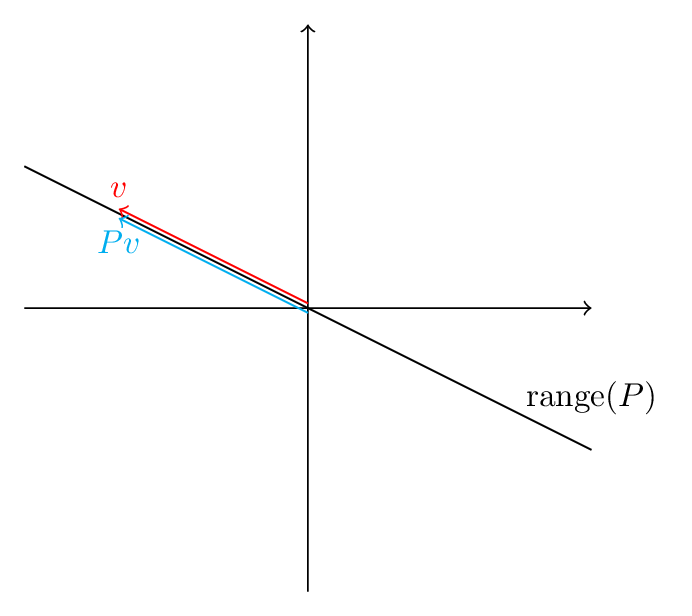
\includegraphics[width=\textwidth]{imgs/inline.png}
    \caption{$v \in \text{range}(P)$}%
    \label{inrange}
    \end{subfigure}
    \hfill
    \begin{subfigure}[b]{0.5\textwidth}
      \centering
      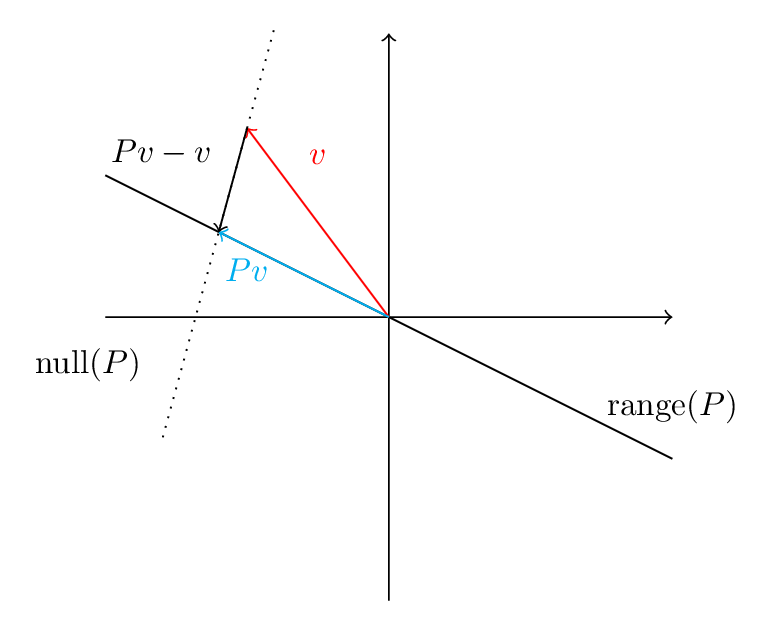
\includegraphics[width=\textwidth]{imgs/outrange.png}
      \caption{$v \notin \text{range}(P)$}
      \label{outrange}
    \end{subfigure}
    \caption{Projecting $v$ with projector $P$}
  \end{figure}
\end{itemize}
Then consider the \textbf{complementary projector} $I - P$:
\begin{itemize}
  \item It's a projector as well. i.e. $(I - P)^2 = I - P$, and simply
    \[
      Pu = 0 \implies (I - P)u = u - Pu = u
    .\]
  \item The proposition above shows that, if a vector $u \in \text{null}(P)$, it is in $\text{range}(I - P)$. To generalize this, we have:
    \[
      [\forall u \in \text{null}(P) \implies \text{range}(I - P)] \implies
    \]
    \[
      \text{null}(P) \subseteq \text{range}(I - P)
    .\] 
    In other words, the nullspace of $P$ is contained in the range of $I - P$.
  \item We could also prove
    \(
      \text{range}(I - P) \subseteq \text{null}(P)
    \) by a similar approach.
    \item And this leads to the result
      \[
        \text{null}(P) = \text{range}(I - P)
      .\]
      similarly
      \[
        \text{null}(I - P) = \text{range}(P)
      .\] 
\end{itemize}
Important things for projector $P$: 
\begin{itemize}
\item  It separates $\mathbb{C}^{m}$ into two spaces, range($P$) and null($P$), where 
  \[
  \text{range}(P) \cap \text{null}(P) = \{\textbf{0}\}
  .\] 
  The reason of why the intersection contains $\textbf{0}$ only is that, considering the two sets $\text{null}(P)$ and $\text{null}(I - P)$, the only common element is $\textbf{0}$. That is because any vector $v$ in both sets satisfies $v = v - Pv = (I - P)v = 0$. And since we know $\text{null}(I - P) = \text{range}(P)$, the results could be shown as stated above. 

\item Conversely, if there exists two subspaces $S_1$ and $S_2$ of $\mathbb{C}^{m}$, where $S_1 \cap S_2 = \{\textbf{0}\}$, there exists a projector $P$ whose range is $S_1$ and nullspace is $S_2$. The proof is not examinable, but it would be better to have a try.
\end{itemize}
% \subsubsection*{Proof}%
% \begin{itemize}
%   \item The proposition above states that, any vector in $\mathbb{C}^{m}$ could be split into two components, in subspaces $S_1$ and $S_2$ respectively.
%   \item Therefore, to prove this proposition, we could simplify this problem to the following proposition:
%     \[
%     \text{Given that } S_1 \cap S_2 = \{0\}, \forall v \in \mathbb{C}^{m}, \text{ find } v_1 \in S_1, v_2 \in S_2: v_1 + v_2 = v 
%     .\]
%     where the projection $Pv$ gives $v_1$ and the complementary projection $(I - P)v$ would gives $v_2$.
%   \item We could find the vector pair since these two subspaces are distinct. But is the vector pair $(v_1, v_2)$ unique?
%   \item Suppose there exists another vector pair $(v_1', v_2') \in S_1 \times S_2$ which satisfies the conditions above, where clearly $v_i \neq v_i'$ and:
%     \[
%       \begin{array}{l}
%       v_1 + v_2 = v \\
%       v_1' + v_2' = v
%       \end{array}
%     .\] 
% \item Subtract the first equation by the second, and we get:
%   \[
%     (v_1 - v_1') + (v_2  - v_2') = \textbf{0} 
%   .\] 
% \item Say $v_1'' = v_1 - v_1'$ and $v_2'' = v_2 - v_2'$, and we could clearly see $v_i'' \in S_i$ due to the properties of subspaces. And we could get that:
%   \[
%   v_1'' + v_2'' = \textbf{0} \implies v_1'' = -v_2''
%   .\]
%  \item We know that the subspace preserves scalar multiplication, therefore, we could see $v_1''$ is in $S_2$ and  $v_2''$ is in $S_1$ as well.
%   \item In this case, we know that $v_1'', v_2''$ are both in $S_1, S_2$. So we could interpret $v_1'', v_2'' \in S_1 \cap S_2 = \{\textbf{0}\} $.
%   \item Then obviously $v_1'' = v_2'' = \textbf{0}$, and
%     \[
%       \begin{array}{l}
%       v_1'' = v_1 - v_1' = \textbf{0} \\
%       v_2'' = v_2 - v_2' = \textbf{0} \\
%       \end{array}
%     \implies 
%       \begin{array}{l}
%       v_1 = v_1' \\
%       v_2 = v_2'
%       \end{array}
%     .\]
%     which contradicts our assumption $v_i \neq v_i'$, so the vector pair $(v_1, v_2)$ should be unique.
%     \item Therefore, we could find a unique decomposition of $v$ into two components $v_1, v_2$ in  $S_1$ and $S_2$. 
%     \item Since we take $v$ arbitrarily, and the components  $v_1, v_2$ in corresponding subspaces $S_1, S_2$ could be written as $Pv$ and  $(I - P)v$ for all chosen $v$, (which are both \textbf{bijection}). So we could say there exists a projector  $P$ such that range$(P) = S_1$ and null$(P) = S_2$.
% \end{itemize}


\section{Orthogonal Projectors and Construction}%
We have known the definition of projectors, but how about orthogonal projectors? The definition states that a projector $P$ is orthogonal if:
\begin{definition}[Orthogonal Projector]
  \[
  \forall v \in \mathbb{C}^{m}, (Pv)^{*}(Pv - v) = 0
  .\] 
\end{definition}
This definition might still be too abstract, so we put the definition into the following \autoref{orthogproj}:
  \begin{figure}[H]
    \centering
    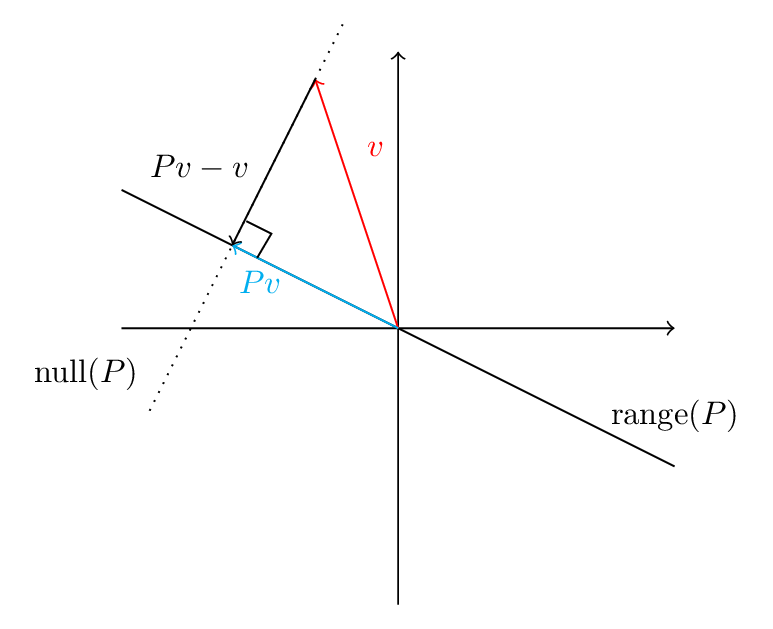
\includegraphics[width=0.6\textwidth]{imgs/orthogonal_proj.png}
    \caption{Projecting $v$ with Orthogonal Projector $P$}
    \label{orthogproj}
  \end{figure}

\noindent We could see the projector $P$ splits $v$ into two components,  $Pv$ and  $Pv - v$. However, in this case, these two components are orthogonal to each other, and computationally, their inner product should be 0. That's where the definition of  \textbf{orthogonal} projector comes from. 
\begin{corollary}
  An orthogonal projector \(P\) splits a vector space e.g.$\mathbb{C}^{m}$ into two orthogonal subspaces, range$(P)$ and null$(P)$.
\end{corollary}

\noindent Then we should have a look at how to construct an orthogonal projector \textbf{from a set of orthonormal vectors.} 

\begin{prop}[Construction of an Orthogonal Projector]
  \[
    \hat{Q} \text{ unitary}, \hat{Q} = \begin{pmatrix} q_1 & q_2 & \ldots & q_n \end{pmatrix} \in \mathbb{C}^{m \times n}, P = \sum_{i=1}^{n} (q_iq_i^{*}) 
  \]
  \[
    \Rightarrow P \text{ is an orthogonal projector} 
  .\]
\end{prop}
\begin{itemize}
\item From the knowledge we get in \href{https://comp-lin-alg.github.io/L1_preliminaries.html#constructing-orthogonal-projectors-from-sets-of-orthonormal-vectors}{section 1.10} master notes, we know that, given we have a set of orthonormal vectors $\{q_1, q_2, \ldots, q_n\}$, for all vector $v \in \mathbb{C}^{m}$, we could write $v$ in terms of:
  \[
    v = r + \sum_{i = 1}^{n} (q_iq_i^{*})v
  .\] 
\item Indeed the context of the proposition fits the formula, and we could see \(r\) and \(\sum_{i=1}^{n} (q_iq_i^{*})\) are orthogonal to each other.  
  \item So if we consider $P = \sum_{i=1}^{n} (q_iq_i^{*})$, then we have:
    \[
    v = r + Pv
    .\] 
    and in this case, each \(P\) could split any \(v \in \mathbb{C}^{m}\) as two components \(Pv\) and \(r = v - Pv = (I - P)v\), and the two components are orthogonal to each other as stated above. 
  \item Then from the definition of orthogonal projectors, we should be confident to say \(P = \sum_{i=1}^{n} (q_iq_i^{*})\) is indeed an orthogonal projector.  
\end{itemize}
The construction looks good, but we have a more concise and elegant way to construct an orthogonal projector.
\newpage
\begin{corollary}[Construction of an Orthogonal Projector, simplified]
  \[
  \hat{Q} \text{ unitary}, P = \hat{Q}\hat{Q}^{*} \Rightarrow P \text{ is an orthogonal projector}
  .\] 
\end{corollary}
% \subsubsection*{Proof}%
\begin{itemize}
  \item Let us say we have $\hat{Q} = \begin{pmatrix} q_1 & q_2 & \ldots & q_n \end{pmatrix} \in \mathbb{C}^{m \times  n}$.
\item We could compute the value of $\hat{Q}\hat{Q}^{*}$ and see that:
  \[
    \hat{Q}\hat{Q}^* = \begin{pmatrix} q_1 & q_2 & \ldots & q_n \end{pmatrix} \begin{pmatrix} q_1^{*}\\ q_2^{*} \\\vdots\\ q_n^{*} \end{pmatrix} = q_1q_1^* + q_2q_2^* + \ldots + q_nq_n^{*} =  \sum_{i=1}^{n} (q_iq_i^{*})
  .\]
  which is exactly what an orthogonal projector \(P\) should be.
  \item So here we conclude that an orthogonal project could be constructed by \textbf{the multiplication of a unitary matrix \(\hat{Q}\) and its adjoint.}
%   see in the construction of the orthogonal projector $P$. \textbf{Personally I think all of you should understand the proof at this level.}

% \item Also, in the light of the change of basis, the product $\hat{Q}^*v$ gives the coefficients of $v$ after projecting along the columns of  $\hat{Q}$, and the multiplication of $\hat{Q}$ on $\hat{Q}^*v$ gives the projections of $v$ expanded in the canonical basis. 
%   \item Therefore, the multiplication by $\hat{Q}\hat{Q}^*$ does the same job as the orthogonal projector $P$ does. We could finally confirm that the orthogonal projectors have a simple form  $P  = \hat{Q}\hat{Q}^{*}$. 
%   \item \textbf{Note:} the last two parts of the proof are mentioned under \textbf{Theorem 1.28 master notes}, and I think it is not necessary to memorise by heart but would give you a deeper understanding if you digest them.
\end{itemize}
Since any orthogonal projector has the form $P = \hat{Q}\hat{Q}^*$, we could see its adjoint $P^* = (\hat{Q}\hat{Q}^*)^* = (\hat{Q}^*)^*(\hat{Q})^* = \hat{Q}\hat{Q}^* = P$. And here is another theorem helping you identify if a projector \(P\) is orthogonal or not:
\begin{theorem}[Orthogonality of Projectors]
  \[
    P^* = P \iff P  \text{ is orthogonal}
    .\]
\end{theorem}
\begin{itemize}
\item We could trivially see the proof of the backwards proposition from the computation above.
\item To prove the forward proposition, we choose a vector $v \in \mathbb{C}^{m}$ arbitrarily, and we have:
  \[
    (Pv)^{*}(Pv - v) = v^*P^*(P - I)v = v^*P(P - I)v 
  \]
  \[
  = v^*(P^2 - P)v = v^*(P - P)v = 0 
  .\] 
  Therefore $P$ is orthogonal.
\end{itemize}

\subsection*{Exercise 1.30 Constructing Orthogonal Projectors}
\addcontentsline{toc}{subsection}{Exercise 1.30 Constructing Orthogonal Projectors}
\subsubsection*{Problem Description}%
This exercise is a relatively easy one - given an orthonormal set of vectors $Q$, we need to implement a function \href{https://comp-lin-alg.github.io/cla_utils.html#cla_utils.exercises2.orthog_proj}{\texttt{exercises2.orthog\_proj()}} to compute an orthogonal projector $P$, which projects vectors to the subspace spanned by elements of  $Q$.
\subsubsection*{What to do}%
We just need to use the construction of an orthogonal projector $P = \hat{Q}\hat{Q}^*$, and in this exercise, we can easily use our provided $Q$ and solve everything. The code implementation should be straightforward enough. \medskip

\noindent \textbf{Remember to check your implementation passes the provided test cases.}
\subsubsection*{What happens next}%
\noindent After learning all the basic things in this chapter, the exciting things finally will come in the following chapters \ldots! The next chapter would be based on the knowledge of orthogonal projectors and we would talk about \textbf{QR factorisation}. 

\bigskip

\begin{center}
  \textit{\large \st{End of Week 2} (we haven't finished this week yet!)} \\
  \medskip
  \textit{\large End of Chapter 1}
\end{center}




